\section{O uwarunkowaniu zadania - inaczej}
%%%%%%%%%%%%%%%%
\begin{frame}{Jakościowo}
	Układ dwóch równań graficznie: \\
    niezależnie od jakości ołówka (algorytm) - lewa strona - dokładniej.
    
    \vspace{.5cm}
    \begin{columns}
    \column{.5\linewidth}
    	\centering   
\includegraphics[width=.7\linewidth]{img/2/2_2_well_conditioned}
    \column{.5\linewidth}
    	\centering   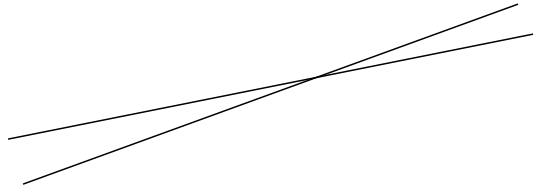
\includegraphics[width=.7\linewidth]{img/2/2_3_ill_conditioned}
    \end{columns}
    \vspace{.5cm}
    \begin{columns}
    \column{.5\linewidth}
    	\centering   well conditioned
    \column{.5\linewidth}
    	\centering   ill conditioned
    \end{columns}
\end{frame}
%%%%%%%%%%%%%%%%
\begin{frame}{Ilościowo}

	{\it Zadanie:} wyznaczenie $f(x)$,\ przy założeniu: $x^{*}$ - blisko $x$ \\
	$\newline$
    Współczynnik uwarunkowania:
    
    \vspace{.5cm}
    \centering
    \begin{tabular}{r c}
    	ogólnie: & \(
            K(x) = \lim_{x^{*} \to x} \frac{
                \left| \frac{
                    f(x) - f(x^{*})
                }{
                    f(x)
                } \right|
            }{
                \left| \frac{
                    x - x^{*}
                }{
                    x
                } \right|
            } = \left| \frac{
                x \cdot f'(x)
            }{
                f(x)
            } \right|
        \)\\
        
        $f(x) = \sqrt{x}$: & \(
        	K(x) = \left| \frac{
                x \cdot \frac{1}{2 \sqrt{x}}
            }{
                \sqrt{x}
            }\right| = \frac{1}{2}
        \) \\
        
        $f(x) = \frac{1}{1 - x}$: & \(
            K(x) = \frac{ \left|
                x \cdot \frac{1}{
                    (1-x)^2
                } \right| 
            }{ \left| 
                \frac{1}{1 - x}
            \right| } = \frac{x}{1 - x}
          	\) \\
            & \(
            x = (1 + 10^{-6}) \Rightarrow K \approx 10^6 \hspace{.5cm} (!)
            \)
    \end{tabular}
\end{frame}
%%%%%%%%%%%%%%%%